
\documentclass{beamer}

\usepackage[german]{babel}
\usepackage[utf8]{inputenc}
\usepackage{pdfpages}

\usetheme{CambridgeUS}


\title[Distanzerhaltende Approximation]{Distanzerhaltende Approximation von Kantenzügen}
\author[N. Klug]{Nikolas Klug}
\institute[Uni Augburg]{Universität Augsburg}
\date{17. Mai 2018}


\begin{document}
	\frame{\titlepage}
	
	\begin{frame}{Einführung in die Problemstellung}
		z.B. Google-maps bilder
		
	\end{frame}
	
	\begin{frame}{Beispiel Approximation}
		Was soll das Ergebnis sein?
		
		Bild aus Arbeit
		
		 + Ergebnis des Beispiels
	\end{frame}
	
	\begin{frame}{Definition t-distanzerhaltend / t-distanzerhaltende Approximation}
		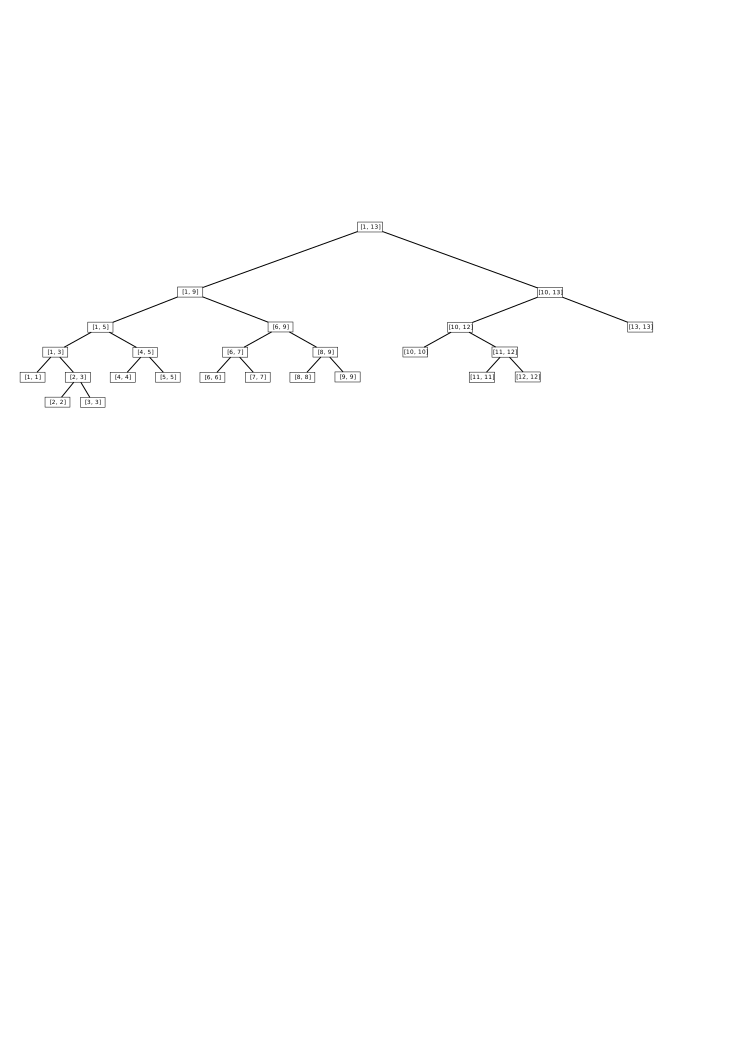
\includepdf[pages={1}]{split_tree_example.pdf}
		
	\end{frame}
	
	\begin{frame}{Problemspezifikation}
		Definition MVPS
		
		Definition MDPS
	\end{frame}
	
	\begin{frame}{Exakter Algorithmus MVPS}
		Konstruktion des Graphen
		
		+ Bild von Beispiel
		
	\end{frame}
	
	\begin{frame}{Exakter Algorithmus MVPS}
		Breitensuche zur Lösung des SSSP-Problems
		
		+ eingezeichneter kürzester Pfad im Beispiel
		
		Frage ans Publikum: Algorithmen zur Lösung des SSSP-Problems
	\end{frame}
	
	\begin{frame}{Exakter Algorithmus MVPS}
		Laufzeitbetrachtung und Satz
	\end{frame}
	
	\begin{frame}{Exakter Algorithmus MDPS}
		kurze Wdh MVPS (evtl. grobe Definition)
		
		Lemma: indirekte Proportionalität kappa und t
		
		kurzer Beweis / Beweiserläuterung
		
		evtl. Frage ans Publikum, da einfach
	\end{frame}
	
	\begin{frame}{Exakter Algorithmus MDPS}
		Bildung der Menge aller t-Werte (Größe $O(n^2)$)
		
		Binäre Suche möglich wegen Lemma
		
	\end{frame}
	
	\begin{frame}{Exakter Algorithmus MDPS}
		Laufzeitbetrachtung
		
		+ evtl. Beispielergebnis
	\end{frame}
	
	\begin{frame}{WSPD}
		Definition Well-separated
		
		+ Beispiel Bild
	\end{frame}
	
	\begin{frame}{WSPD}
		Definition WSPD
		
		+ Beispiel Bild (zweidimensional und evtl. mit den Werten aus unserem Beispiel)
	\end{frame}
	
	\begin{frame}{WSPD - Algorithmus}
		Erklärung Split-Tree (binärer Baum)
		
		+ Beispiel mit unseren Werten
	\end{frame}
	
	
	\begin{frame}{WSPD - Algorithmus}
		Satz: Laufzeit
		
		Algorithmus nicht wichtig, nachlesen in Arbeit für Interessierte
		
		Aber wichtig: Die WSPD Mengen werden durch Knoten des Split-Trees repräsentiert, wobei ein Knoten mehrere Mengen repräsentieren kann
	\end{frame}
	
	\begin{frame}{Approximativer Algorithmus WSPD}
		Sei $\epsilon = $..., $s = $ ...
		
		Lemma: 	t-distanzerhaltend $=>$ 1 + e/3 t-distanzerhaltend
				1 + e/3 t-distanzerhaltend $=>$ 1 + e t-distanzerhaltend
				
		+ zweidimensionale Beispiele
	\end{frame}
	
	\begin{frame}{Approximativer Algorithmus WSPD}
		Konstruktion des Graphen H aus "Knoten" der WSPD
		
		Knoten: Elemente der WSPD
		
		Kanten: "?"
	\end{frame}
	
	\begin{frame}{Approximativer Algorithmus WSPD}
		Kanten:
		
		Definition
		
		+ Beispiele
	\end{frame}
	
	\begin{frame}{Approximativer Algorithmus WSPD}
		Satz: Jede Approximation entspricht einem Pfad in H
		
		Beweisskizze
	\end{frame}
	
	\begin{frame}{Approximativer Algorithmus WSPD}
		Satz: Jeder Pfad in H entspricht einer Approximation
	\end{frame}
\end{document}